
\section{Experimental results}
\label{sec:experiments}

In this section we present a set of experiments designed to evaluate different aspects of \FAMA, from its performance to the quality of the learned models. Whenever applicable, we will consider both NP-complete and PSPACE-complete scenarios, in order to draw conclusions at both levels of complexity. We will also devote one experiment to assess the suitability of the evaluation metrics proposed in this paper. 

\subsection{Setup}
We evaluate \FAMA on fourteen IPC domains that satisfy the \strips\ requirement~\cite{fox2003pddl2} and that are taken from the {\sc planning.domains} repository~\cite{muise2016planning}. Table \ref{tab:domain_features} compiles the features of these fourteen domains used in the experiments. From left to right, the columns report the name of the domain, number of actions, number of predicates, maximum arity of the actions, and maximum arity of the predicates. These are all features which affect the size of $P_\Lambda$ and hence, have an impact on the complexity of the learning task. %As can be seen in table \ref{tab:domain_features}, the selected domains range from, such as \emph{blocks} and \emph{visitall}, to complex ones, like \emph{floortile} and \emph{satellite}, with higher number of actions and predicates and with higher arity.

In the following, we explain the details of our experimental setup:

\begin{itemize}

\item {\bf Plan traces}. For each domain, we have generated 10 plan traces with 10 actions/intermediate states each using random walks. Depending on the experiment, these traces are used for training or testing, so more details will be provided later.

\item {\bf Planner}. The classical planner we use to solve the $P_\Lambda$ instances that result from our compilations is {\sc Madagascar}~\cite{rintanen2014madagascar}. We use {\sc Madagascar} for two reasons: 1) its ability to deal with planning instances populated with dead-ends, and 2) when the length of the plan traces is known (\FO action sequences or \FO state trajectories), the horizon of the solution plan is also known and can be provided to {\sc Madagascar}, addressing in this case NP-complete problems. This is because, SAT-based planners can apply the actions for programming preconditions in parallel during a single planning step (and the same for actions programming effects) because these actions do not interact. Hence, we know that the programming prefix of the solution plan can be solved in two steps, independently of the number of programming actions applied.

\item {\bf Machine}. All experiments are run on an Intel Core i5 3.50 GHz x 4 with 16 GB of RAM.

\item {\bf Reproducibility}. We make fully available the compilation source code, the evaluation scripts and the used benchmarks at this repository {\em https://github.com/sjimenezgithub/strips-learning} so any experimental data reported in the paper is fully reproducible.
\end{itemize}

\begin{table}[hbt!]
		\begin{center}
			\begin{tabular}{l|c|c|c|c|}	
				& \multicolumn{4}{c|}{Domain features}\\ \cline{2-5}
				 & {\bf \# actions} & {\bf \# predicates} & {\bf max action arity} & {\bf max predicate arity}  \\
				\hline
				Blocks & 4 & 5 & 2 & 2  \\
				Driverlog & 6 & 5 & 4 & 2  \\
				Ferry & 3 & 5 & 2 & 2  \\
				Floortile & 7 & 10 & 4 & 2  \\
				Grid & 5 & 9 & 4 & 2  \\
				Gripper & 3 & 4 & 3 & 2  \\
				Hanoi & 1 & 3 & 3 & 2  \\
				Miconic & 4 & 6 & 2 & 2  \\
				Npuzzle & 1 & 3 & 3 & 2  \\
				Parking & 4 & 5 & 3 & 2  \\
				Satellite & 5 & 8 & 4 & 2  \\
				Transport & 3 & 5 & 5 & 2  \\
				Visitall & 1 & 3 & 2 & 2  \\
				Zenotravel & 5 & 4 & 5 & 2
			\end{tabular}
		\end{center}
	\caption{\small Feature description of the 13 domains used in the experiments.}
	\label{tab:domain_features}	
\end{table}

\subsection{Impact of the size of the input knowledge}
This experiment evaluates how the size of the input knowledge, i.e., $\left|\mathcal{T}\right|$ affects the performance of \FAMA. The experiment analyzes the evolution of the computation time as well as the quality of the learned models as the size of $\mathcal{T}$ increases (from 1 to 10). Recall that each trace in $\mathcal{T}$ comprises 10 actions/intermediate states. To keep the experiment practicable, we introduce a 1000s timeout after which the learning process is killed and the learned models are assigned a score of 0 for both precision and recall. Our goals with this experiment are to:
\begin{enumerate}
	\item Identify the amount of input required by \FAMA to learn sound and complete models,
	\item Evaluate the scalability of \FAMA wrt the input size which, as stated in section \ref{sec:properties}, is one of the limiting factors of our approach.
\end{enumerate} 

With this in mind we defined two case studies:
\begin{itemize}
	\item \textbf{\FO action sequence and \PO state trajectory}: This is the typical case addressed by most previous work, which corresponds to a NP-complete scenario. We are assuming a degree of observability of just 10\% for the state trajectory, meaning that each literal of a state has a 10\% chance of being observed.
	\item  \textbf{\NO action sequence and \NO state trajectory}: This is a PSPACE-complete scenario where both the action sequence and state trajectory are completely empty and only initial and final states are observed, i.e., $\tau = \tup{s_0, s_m}, \forall \tau \in \mathcal{T}$.
\end{itemize}

\begin{figure}[hbt!]
	\centering
	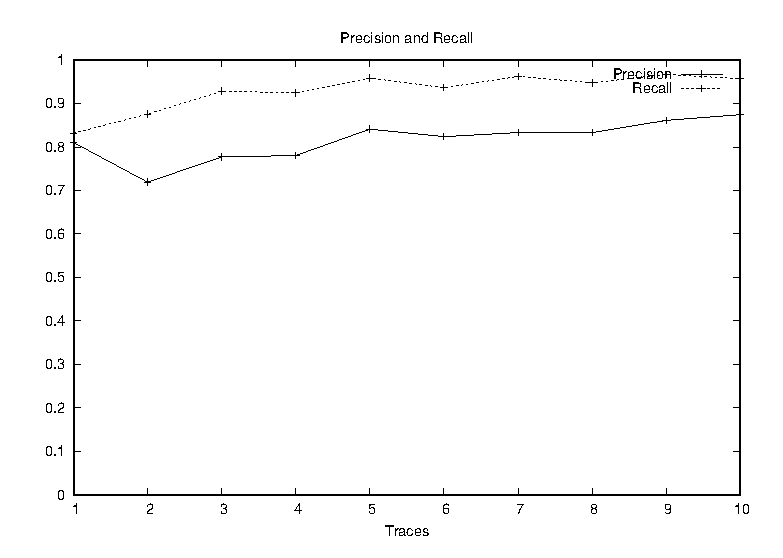
\includegraphics[width=0.8\linewidth]{figures/input_size_100_10_precision.eps}
	\caption{Evaluation of the impact of the input size on the quality of the learned models when learning from plan traces with \FO action sequences and \PO state trajectories with 10\% observability}
	\label{fig:np_quality}
\end{figure}

\begin{figure}[hbt!]
	\centering
	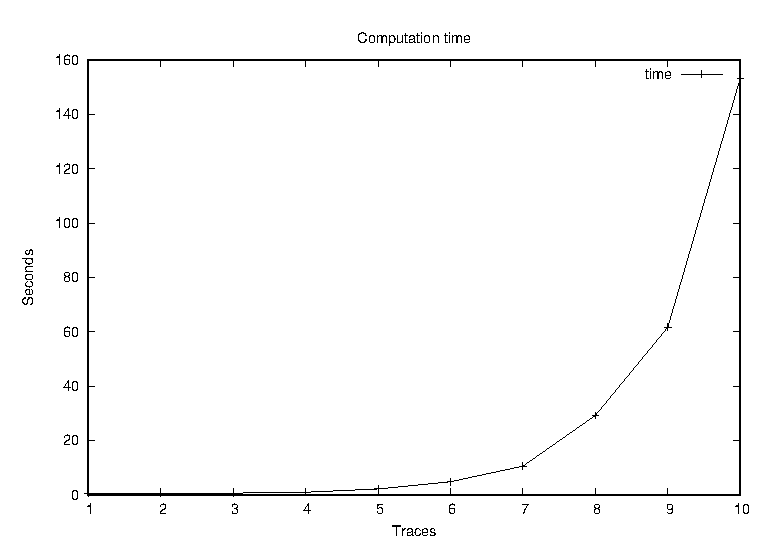
\includegraphics[width=0.8\linewidth]{figures/input_size_100_10_time.eps}
	\caption{Evaluation of the impact of the input size on the computation time when learning from plan traces with \FO action sequences and \PO state trajectories with 10\% observability}
	\label{fig:np_time}
\end{figure}

Figures \ref{fig:np_quality} and \ref{fig:np_time} show the quality of the models and computation time, respectively, for the NP-complete scenario. In figure \ref{fig:np_quality} we see precision stabilizes at 0.86 after 5 traces while recall stabilizes at 0.95 after 3 traces. These results show that \FAMA does, in fact, not need big amounts of input to learn sound and complete models as opposite to other approaches in the literature where models are learned using around a hundred traces (see table \ref{table:models_comparison2}).

With regards to the scalability of \FAMA, figure \ref{fig:np_time} paints a very interesting picture. In this figure, we can see an exponential increase in computation time for input sizes beyond 5 traces. Until an input size of 4 traces the computation time is below 1 s, but it reaches 153 s when the input is composed of 10 traces. These results match the performance of {\sc Madagascar}, since this planner is known to struggle with plan horizons beyond 150-200 steps (in our case 160 steps corresponds to 8 traces).


\begin{figure}[hbt!]
	\centering
	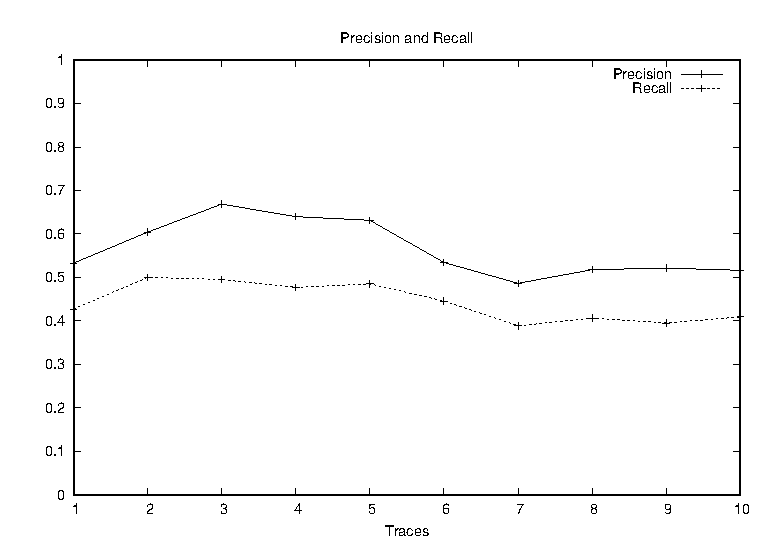
\includegraphics[width=0.8\linewidth]{figures/input_size_0_0_precision.eps}
	\caption{Evaluation of the impact of the input size on the quality of the learned models when learning from plan traces with \NO action sequences and \NO state trajectories}
	\label{fig:pspace_quality}
\end{figure}

\begin{figure}[hbt!]
	\centering
	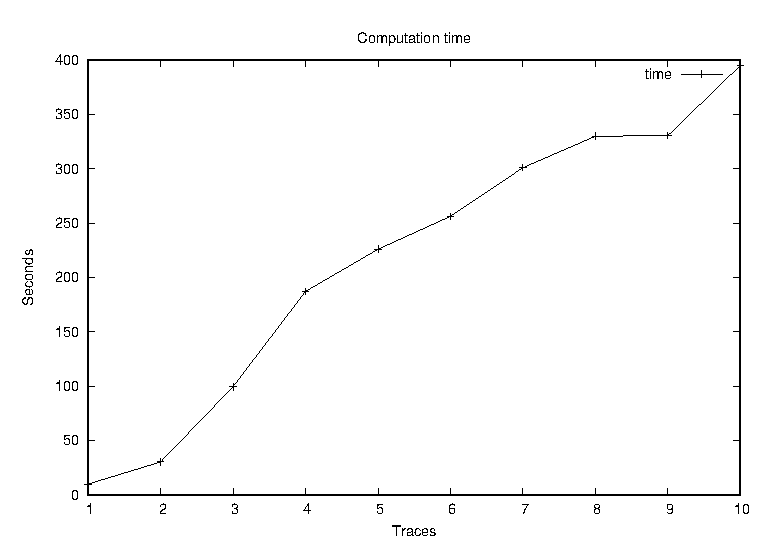
\includegraphics[width=0.8\linewidth]{figures/input_size_0_0_time.eps}
	\caption{Evaluation of the impact of the input size on the computation time when learning from plan traces with \NO action sequences and \NO state trajectories}
	\label{fig:pspace_time}
\end{figure}

Next, we evaluate the PSPACE-complete scenario. As expected, the quality of the learned models, shown in figure \ref{fig:pspace_quality}, is inferior than in the NP-complete case. The results contradict the previous trend and we find a drop in quality as the input knowledge increases. This is, in fact, caused by an increasing number of timeouts in the experiments, meaning that no solution is found. The computation time in this scenario (figure \ref{fig:pspace_time}) is also considerably higher given the complexity of the task, which is reflected on the amount of timeouts.

The conclusion we can draw is that learning from few input samples is both our strong point and our limitation. Results on the NP-complete scenario show that the learned models are considerably sound and complete (to put these results into a richer perspective we will also compare ourselves with another approach in the following section). The PSPACE-complete scenario, on the other hand, shows that the learned models have less quality. Nevertheless, we argue that syntax-based metrics are not appropriate for the PSPACE-complete scenario due to the vast amount of reformulations that can appear in such under-constrained learning task and we will show proof of this in section \ref{minimal}.


\subsection{Comparison with \ARMS}
Here we compare the performance of \FAMA to that of \ARMS, one of the most well-known approaches learning planning models. \ARMS works under the assumption of plan traces with \FO action sequences and \NO state trajectories, so we will also adopt this assumption (\ARMS, as any other previous approaches for learning planning models cannot handle the PSPACE-complete scenarios).

We define a \emph{degree of observability} $\sigma$ for the state trajectory, ranging from 0\% to 100\%, that measures the probability of observing a literal, and evaluate both approaches as $\sigma$ increases using 5 plan traces as input. Note that when $\sigma = 0$ we have a \NO state trajectory, when $\sigma=100$ we have a \FO state trajectory and all cases in-between correspond to the \PO scenario. Figures \ref{fig:comparison_precision} and \ref{fig:comparison_recall} compare \FAMA and \ARMS in terms of precision and recall. The horizontal axis represents the degree of observability, while the vertical axis show the average precision (figure \ref{fig:comparison_precision}) or recall (figure \ref{fig:comparison_recall}) computed over the fourteen tested domains. Remarkably, figure \ref{fig:comparison_precision} shows that \FAMA dominates in terms of precision in all cases save for \FO state trajectories. Furthermore, in average, the models learned by our approach are 15\% to 24\% more precise than those learned by \ARMS. A similar conclusion can be drawn for recall (figure \ref{fig:comparison_recall}), where the difference is even larger, meaning that our models are more complete.

\begin{figure}[hbt!]
	\centering
	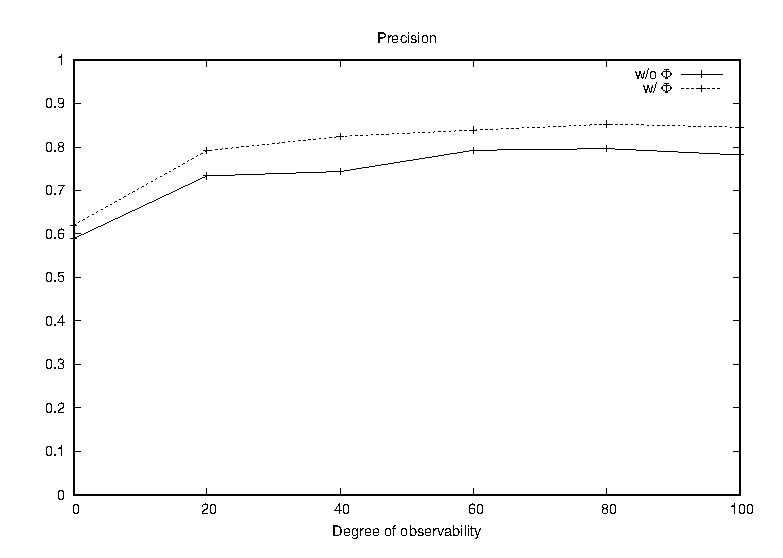
\includegraphics[width=.8\linewidth]{figures/comparison_precision.eps}
	\caption{Precision comparison between \FAMA and \ARMS}
	\label{fig:comparison_precision}
\end{figure}

\begin{figure}[hbt!]
	\centering
	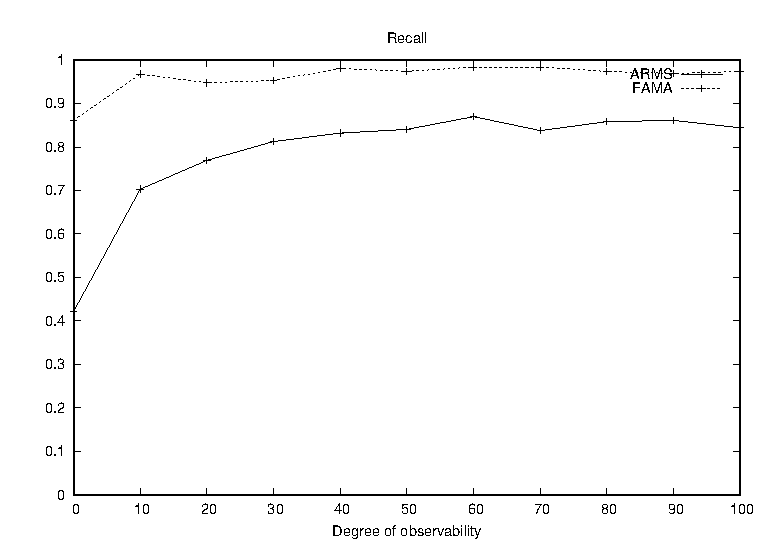
\includegraphics[width=.8\linewidth]{figures/comparison_recall.eps}
	\caption{Recall comparison between \FAMA and \ARMS}
	\label{fig:comparison_recall}
\end{figure}



%Remarkably, the overall \emph{precision} is now $0.98$, which means that the contents of the learned models is highly reliable. The value of \emph{recall}, 0.87, is an indication that the learned models still miss some information (preconditions are again the component more difficult to be fully learned). Overall, the results confirm the previous trend: the more input knowledge of the task, the better the models and the less planning time. Additionally, the solution plans required for this task are smaller because it is only necessary to program half of the actions (the other half are included in the input knowledge $\mathcal{M}$). {\em Visitall} and {\em Hanoi} are excluded from this evaluation because they only contain one action schema.

\FAMA outperforms \ARMS in this particular experiment, which is one with very limited input. By no means do these results imply that our approach is overall better for the NP-complete scenarios, just that it is able to learn better models when few plan traces are available. We are not reporting experiments where far more input traces are available, since \FAMA cannot handle so much input.



\subsection{Experiments with minimal input knowledge}
\label{minimal}
%In the previous experiments we have given a general view of the performance of \FAMA under different conditions.
So far, experiments have shown that \FAMA is able to learn with very small amounts of input knowledge, be it due to low observability or few training samples. In this section we want to take a closer look at the action models learned from minimal input knowledge. To that end, we will limit the input to only 2 plan traces and analyze the results under different levels of observability.

In this experiment we evaluate three case studies, the first one being an NP-complete scenario and the other two being PSPACE-complete:
\begin{itemize}
	\item \textbf{\FO action sequence and \PO state trajectory}: We are, once again, assuming a degree of observability of 10\% for the state trajectory. The results of this case study are detailed in table \ref{tab:results_minimum_100_10}
	\item  \textbf{\PO action sequence and \PO state trajectory}: In this case study we are assuming a degree of observability of 30\% for both the action sequence and state trajectory. The results of this case study are detailed in table \ref{tab:results_minimum_30_30}
	\item  \textbf{\NO action sequence and \NO state trajectory}: Both the action sequence and state trajectory are completely empty and only initial and final states are observed, i.e., $\tau = \tup{s_0, s_m}, \forall \tau \in \mathcal{T}$. The results of this case study are detailed in table \ref{tab:results_minimum_0_0}
\end{itemize}

All tables in this section (tables \ref{tab:results_minimum_100_10}, \ref{tab:results_minimum_0_0}, \ref{tab:results_minimum_30_30}) follow the same structure. In these tables precision ({\bf P}) and recall ({\bf R}) are computed separately for the preconditions ({\bf Pre}), positive effects ({\bf Add}) and negative Effects ({\bf Del}), and also globally ({\bf Global}). The last column reports the computation time in seconds needed to obtain the learned models. Missing values in the tables correspond to domains where no solution was found given a timeout of 1800 s.

\begin{table}[hbt!]
		\begin{center}
			
			\begin{tabular}{l|l|l|l|l|l|l||l|l|l|}
				& \multicolumn{2}{|c|}{\bf Pre} & \multicolumn{2}{|c|}{\bf Add} & \multicolumn{2}{|c||}{\bf Del} & \multicolumn{2}{|c|}{\bf Global} & \\ \cline{2-9}			
				& \multicolumn{1}{|c|}{\bf P} & \multicolumn{1}{|c|}{\bf R} & \multicolumn{1}{|c|}{\bf P} & \multicolumn{1}{|c|}{\bf R} & \multicolumn{1}{|c|}{\bf P} & \multicolumn{1}{|c||}{\bf R} &  \multicolumn{1}{|c|}{\bf P} & \multicolumn{1}{|c|}{\bf R} & {\bf Time} \\
				\hline
				blocks & 0.86 & 0.67 & 0.86 & 0.67 & 0.8 & 0.44 & 0.84 & 0.59& 0.21 \\ % [(u'pick-up', u'pick-up', 1), (u'put-down', u'put-down', 1), (u'stack', u'stack', 1, 2), (u'unstack', u'unstack', 1, 2)]
				driverlog & 0.68 & 0.93 & 0.5 & 0.57 & 0.83 & 0.71 & 0.67 & 0.79& 0.27 \\ % [(u'load-truck', u'load-truck', 1, 2, 3), (u'unload-truck', u'unload-truck', 1, 2, 3), (u'board-truck', u'board-truck', 1, 2, 3), (u'disembark-truck', u'disembark-truck', 1, 2, 3), (u'walk', u'walk', 1, 2, 3), (u'drive-truck', u'drive-truck', 1, 2, 3, 4)]
				ferry & 0.78 & 1.0 & 0.5 & 1.0 & 1.0 & 1.0 & 0.71 & 1.0& 0.4 \\ % [(u'sail', u'sail', 1, 2), (u'board', u'board', 1, 2), (u'debark', u'debark', 1, 2)]
				floor-tile & 0.69 & 1.0 & 0.45 & 0.91 & 1.0 & 0.82 & 0.65 & 0.93& 1.42 \\ % [(u'change-color', u'change-color', 1, 2, 3), (u'up', u'up', 1, 2, 3), (u'down', u'down', 1, 2, 3), (u'right', u'right', 1, 2, 3), (u'left', u'left', 1, 2, 3), (u'paint-up', u'paint-up', 1, 2, 3, 4), (u'paint-down', u'paint-down', 1, 2, 3, 4)]
				grid & 0.76 & 0.94 & 0.55 & 0.86 & 1.0 & 1.0 & 0.74 & 0.94& 0.7 \\ % [(u'move', u'move', 1, 2), (u'pickup', u'pickup', 1, 2), (u'putdown', u'putdown', 1, 2), (u'pickup-and-loose', u'pickup-and-loose', 1, 2, 3), (u'unlock', u'unlock', 1, 2, 3, 4)]
				gripper-strips & 1.0 & 1.0 & 1.0 & 1.0 & 1.0 & 1.0 & 1.0 & 1.0& 0.16 \\ % [(u'move', u'move', 1, 2), (u'pick', u'pick', 1, 2, 3), (u'drop', u'drop', 1, 2, 3)]
				hanoi & 0.67 & 1.0 & 0.67 & 1.0 & 1.0 & 1.0 & 0.73 & 1.0& 0.31 \\ % [(u'move', u'move', 1, 2, 3)]
				miconic & 1.0 & 1.0 & 0.5 & 1.0 & 1.0 & 1.0 & 0.8 & 1.0& 0.29 \\ % [(u'board', u'board', 1, 2), (u'depart', u'depart', 1, 2), (u'up', u'up', 1, 2), (u'down', u'down', 1, 2)]
				n-puzzle & 0.75 & 1.0 & 1.0 & 1.0 & 1.0 & 1.0 & 0.88 & 1.0& 0.28 \\ % [(u'move', u'move', 1, 2, 3)]
				parking & 0.73 & 0.79 & 0.7 & 0.78 & 1.0 & 0.78 & 0.78 & 0.78& 0.65 \\ % [(u'move-curb-to-curb', u'move-curb-to-curb', 1, 2, 3), (u'move-curb-to-car', u'move-curb-to-car', 1, 2, 3), (u'move-car-to-curb', u'move-car-to-curb', 1, 2, 3), (u'move-car-to-car', u'move-car-to-car', 1, 2, 3)]
				satellite & 0.93 & 1.0 & 0.63 & 1.0 & 1.0 & 0.75 & 0.85 & 0.96& 0.36 \\ % [(u'switch-on', u'switch-on', 1, 2), (u'switch-off', u'switch-off', 1, 2), (u'turn-to', u'turn-to', 1, 2, 3), (u'calibrate', u'calibrate', 1, 2, 3), (u'take-image', u'take-image', 1, 2, 3, 4)]
				transport & 1.0 & 1.0 & 0.71 & 1.0 & 1.0 & 0.6 & 0.9 & 0.9& 0.22 \\ % [(u'drive', u'drive', 1, 2, 3), (u'pick-up', u'pick-up', 1, 2, 3, 4, 5), (u'drop', u'drop', 1, 2, 3, 4, 5)]
				grid-visit-all & 0.67 & 1.0 & 0.5 & 1.0 & 1.0 & 1.0 & 0.63 & 1.0& 0.87 \\ % [(u'move', u'move', 1, 2)]
				zeno-travel & 0.92 & 0.79 & 0.6 & 0.86 & 0.8 & 0.57 & 0.78 & 0.75& 0.26 \\ % [(u'board', u'board', 1, 2, 3), (u'debark', u'debark', 1, 2, 3), (u'refuel', u'refuel', 1, 2, 3, 4), (u'fly', u'fly', 1, 2, 3, 4, 5), (u'zoom', u'zoom', 1, 2, 3, 4, 5, 6)]
				\hline
				\bf & 0.82 & 0.94 & 0.66 & 0.90 & 0.96 & 0.83 & 0.78 & 0.90 & 0.46 \\
			\end{tabular}
			
		\end{center}
	\caption{\small {\em Precision} and {\em recall} scores for learning tasks with \FO action sequences and \PO state trajectories with 10\% observability}
	\label{tab:results_minimum_100_10}
\end{table}

Table \ref{tab:results_minimum_100_10} shows the results of the first case study. As was expected from the previous experiments, the recall scores are generally higher than the precision ones, and, in fact, the models learned for 6 of the tested domains were perfectly complete. Although precision is overall lower, it is interesting to notice that the soundness of most learned sets of positive effects is flawless. With regards to the computation time, we find times below the second in all cases except for one, "floor-tile", the most complex among the tested domains.

\begin{table}[hbt!]
	\begin{center}
		
		\begin{tabular}{l|l|l|l|l|l|l||l|l|l|}
			& \multicolumn{2}{|c|}{\bf Pre} & \multicolumn{2}{|c|}{\bf Add} & \multicolumn{2}{|c||}{\bf Del} & \multicolumn{2}{|c|}{\bf Global} & \\ \cline{2-9}			
			& \multicolumn{1}{|c|}{\bf P} & \multicolumn{1}{|c|}{\bf R} & \multicolumn{1}{|c|}{\bf P} & \multicolumn{1}{|c|}{\bf R} & \multicolumn{1}{|c|}{\bf P} & \multicolumn{1}{|c||}{\bf R} &  \multicolumn{1}{|c|}{\bf P} & \multicolumn{1}{|c|}{\bf R} & {\bf Time} \\
			\hline
			blocks & 1.0 & 0.89 & 0.9 & 1.0 & 1.0 & 0.89 & 0.96 & 0.93& 3.51 \\ % [(u'pick-up', u'put-down', 1), (u'put-down', u'pick-up', 1), (u'stack', u'stack', 1, 2), (u'unstack', u'unstack', 1, 2)]
			driverlog & 0.3 & 0.21 & 0.31 & 0.57 & 0.29 & 0.29 & 0.3 & 0.32& 24.41 \\ % [(u'load-truck', u'unload-truck', 1, 2, 3), (u'unload-truck', u'load-truck', 1, 2, 3), (u'board-truck', u'board-truck', 1, 2, 3), (u'disembark-truck', u'disembark-truck', 1, 2, 3), (u'walk', u'walk', 2, 1, 3), (u'drive-truck', u'drive-truck', 1, 2, 3, 4)]
			ferry & 0.83 & 0.71 & 0.8 & 1.0 & 1.0 & 1.0 & 0.87 & 0.87& 4.39 \\ % [(u'sail', u'sail', 1, 2), (u'board', u'board', 1, 2), (u'debark', u'debark', 1, 2)]
			floor-tile & - & - & - & - & - & - & - & - & - \\ % [(u'change-color', u'change-color', 1, 2, 3), (u'up', u'change-color', 1, 3, 2), (u'down', u'up', 1, 2, 3), (u'right', u'up', 1, 3, 2), (u'left', u'down', 1, 3, 2), (u'paint-up', u'paint-up', 1, 2, 3, 4), (u'paint-down', u'paint-down', 1, 2, 3, 4)]
			grid & - & - & - & - & - & - & - & - & - \\ % [(u'move', u'move', 1, 2), (u'pickup', u'move', 2, 1), (u'putdown', u'putdown', 1, 2), (u'pickup-and-loose', u'pickup-and-loose', 1, 2, 3), (u'unlock', u'unlock', 1, 2, 3, 4)]
			gripper-strips & 1.0 & 0.67 & 0.8 & 1.0 & 1.0 & 1.0 & 0.92 & 0.86& 1.31 \\ % [(u'move', u'move', 1, 2), (u'pick', u'pick', 1, 2, 3), (u'drop', u'drop', 1, 2, 3)]
			hanoi & 1.0 & 0.5 & 1.0 & 1.0 & 1.0 & 1.0 & 1.0 & 0.75& 1566.44 \\ % [(u'move', u'move', 1, 2, 3)]
			miconic & 0.75 & 0.33 & 0.5 & 0.75 & 0.5 & 0.67 & 0.57 & 0.5& 0.86 \\ % [(u'board', u'board', 1, 2), (u'depart', u'depart', 1, 2), (u'up', u'up', 2, 1), (u'down', u'down', 1, 2)]
			n-puzzle & 1.0 & 1.0 & 1.0 & 1.0 & 1.0 & 1.0 & 1.0 & 1.0& 62.82 \\ % [(u'move', u'move', 1, 2, 3)]
			parking & - & - & - & - & - & - & - & - & - \\ % [(u'move-curb-to-curb', u'move-curb-to-curb', 1, 2, 3), (u'move-curb-to-car', u'move-curb-to-curb', 1, 3, 2), (u'move-car-to-curb', u'move-curb-to-car', 1, 2, 3), (u'move-car-to-car', u'move-car-to-curb', 1, 2, 3)]
			satellite & 0.78 & 0.5 & 0.57 & 0.8 & 0.33 & 0.25 & 0.63 & 0.52& 22.76 \\ % [(u'switch-on', u'switch-on', 1, 2), (u'switch-off', u'switch-off', 1, 2), (u'turn-to', u'turn-to', 1, 2, 3), (u'calibrate', u'calibrate', 1, 2, 3), (u'take-image', u'take-image', 1, 2, 3, 4)]
			transport & 0.5 & 0.3 & 0.43 & 0.6 & 0.5 & 0.4 & 0.47 & 0.4& 31.07 \\ % [(u'drive', u'drive', 1, 2, 3), (u'pick-up', u'pick-up', 1, 2, 3, 5, 4), (u'drop', u'drop', 1, 2, 3, 5, 4)]
			grid-visit-all & 1.0 & 0.5 & 0.5 & 0.5 & 1.0 & 1.0 & 0.75 & 0.6& 3.11 \\ % [(u'move', u'move', 1, 2)]
			zeno-travel & 0.67 & 0.29 & 0.75 & 0.43 & 0.75 & 0.43 & 0.71 & 0.36& 494.2 \\ % [(u'board', u'board', 1, 2, 3), (u'debark', u'debark', 1, 2, 3), (u'refuel', u'refuel', 1, 2, 3, 4), (u'fly', u'fly', 1, 3, 2, 5, 4), (u'zoom', u'zoom', 1, 2, 3, 4, 5, 6)]
			\hline
			\bf & 0.80 & 0.54 & 0.69 & 0.79 & 0.76 & 0.72 & 0.74 & 0.65 & 201.35 
			
		\end{tabular}
		
	\end{center}
	\caption{\small {\em Precision} and {\em recall} scores for learning tasks with \PO action sequences and \PO state trajectories with 30\% observability in both cases}
	\label{tab:results_minimum_30_30}
\end{table}

The first thing to notice in table \ref{tab:results_minimum_30_30}, which collects the result of the PSPACE case study with 30\% observability, is that the values for some domains are missing. This is the case for "floor-tile", and "parking" which not only are fairly complex domains, but are also considered \emph{puzzle-like}, a quality that is known to put a strain on the planners. Interestingly enough, "hanoi" also qualifies as a \emph{puzzle-like} domain, and we can see how this is reflected on the computation time. With regards to the quality of the models, we find that the learned models retain a similar level of soundness, while their completeness has drastically worsened with respect to the previous case study. This is specially the case for the preconditions, which have gone from 0.94 recall to 0.54. %This results are difficult to explain, given that in this case study the intermediate states contain more information, but
Our intuition is that the input actions play a big role on how close the learned model are with respect to the GTM.

Next, we analyze the PSPACE case study with \NO action sequences and state trajectories (Table \ref{tab:results_minimum_0_0}). Contrary to what might be expected by looking at the previous table, we are able to find solutions for all domains. This is because, although the search is less guided, there are far more possible solutions for this learning task. This wider range of solutions is also evidenced by the quality of the learned models, which in spite of being compliant with the input data, are further from the original GTM. In the table we find that both precision and recall have seen their scores decreased to 0.6 and 0.5, respectively. 

\begin{table}[hbt!]
	\begin{center}		
		\begin{tabular}{l|l|l|l|l|l|l||l|l|l|}
			& \multicolumn{2}{|c|}{\bf Pre} & \multicolumn{2}{|c|}{\bf Add} & \multicolumn{2}{|c||}{\bf Del} & \multicolumn{2}{|c|}{\bf Global} & \\ \cline{2-9}			
			& \multicolumn{1}{|c|}{\bf P} & \multicolumn{1}{|c|}{\bf R} & \multicolumn{1}{|c|}{\bf P} & \multicolumn{1}{|c|}{\bf R} & \multicolumn{1}{|c|}{\bf P} & \multicolumn{1}{|c||}{\bf R} &  \multicolumn{1}{|c|}{\bf P} & \multicolumn{1}{|c|}{\bf R} & {\bf Time} \\
			\hline
			blocks & 0.5 & 0.56 & 0.5 & 0.33 & 0.75 & 0.33 & 0.55 & 0.41& 0.27 \\ % [(u'pick-up', u'put-down', 1), (u'put-down', u'pick-up', 1), (u'stack', u'stack', 1, 2), (u'unstack', u'unstack', 1, 2)]
			driverlog & 0.13 & 0.07 & 0.38 & 0.71 & 0.0 & 0.0 & 0.25 & 0.21& 0.98 \\ % [(u'load-truck', u'load-truck', 1, 2, 3), (u'unload-truck', u'unload-truck', 1, 2, 3), (u'board-truck', u'disembark-truck', 1, 2, 3), (u'disembark-truck', u'board-truck', 1, 2, 3), (u'walk', u'walk', 1, 2, 3), (u'drive-truck', u'drive-truck', 1, 2, 3, 4)]
			ferry & 0.5 & 0.29 & 0.5 & 0.5 & 0.67 & 0.5 & 0.55 & 0.4& 0.47 \\ % [(u'sail', u'sail', 1, 2), (u'board', u'board', 1, 2), (u'debark', u'debark', 1, 2)]
			floor-tile & 0.34 & 0.64 & 0.5 & 0.36 & 0.44 & 0.73 & 0.39 & 0.59& 165.92 \\ % [(u'change-color', u'change-color', 1, 2, 3), (u'up', u'up', 1, 3, 2), (u'down', u'left', 1, 2, 3), (u'right', u'right', 1, 3, 2), (u'left', u'left', 1, 3, 2), (u'paint-up', u'paint-up', 1, 3, 2, 4), (u'paint-down', u'paint-down', 1, 3, 2, 4)]
			grid & 0.47 & 0.41 & 0.38 & 0.43 & 0.25 & 0.29 & 0.39 & 0.39& 214.87 \\ % [(u'move', u'move', 1, 2), (u'pickup', u'pickup', 1, 2), (u'putdown', u'putdown', 1, 2), (u'pickup-and-loose', u'pickup-and-loose', 1, 3, 2), (u'unlock', u'unlock', 2, 1, 3, 4)]
			gripper-strips & 1.0 & 0.83 & 1.0 & 1.0 & 1.0 & 1.0 & 1.0 & 0.93& 0.2 \\ % [(u'move', u'move', 1, 2), (u'pick', u'pick', 1, 2, 3), (u'drop', u'drop', 1, 2, 3)]
			hanoi & 0.6 & 0.75 & 1.0 & 1.0 & 1.0 & 1.0 & 0.78 & 0.88& 3.23 \\ % [(u'move', u'move', 1, 3, 2)]
			miconic & 0.4 & 0.44 & 0.6 & 0.75 & 0.25 & 0.33 & 0.42 & 0.5& 0.25 \\ % [(u'board', u'board', 1, 2), (u'depart', u'depart', 1, 2), (u'up', u'up', 2, 1), (u'down', u'down', 2, 1)]
			n-puzzle & 1.0 & 1.0 & 1.0 & 1.0 & 1.0 & 1.0 & 1.0 & 1.0& 4.15 \\ % [(u'move', u'move', 1, 2, 3)]
			parking & 0.67 & 0.57 & 0.43 & 0.33 & 0.5 & 0.44 & 0.56 & 0.47& 7.61 \\ % [(u'move-curb-to-curb', u'move-curb-to-curb', 1, 3, 2), (u'move-curb-to-car', u'move-curb-to-car', 1, 2, 3), (u'move-car-to-curb', u'move-car-to-curb', 1, 2, 3), (u'move-car-to-car', u'move-car-to-car', 2, 1, 3)]
			satellite & 0.5 & 0.14 & 0.5 & 0.6 & 0.75 & 0.75 & 0.57 & 0.35& 2.06 \\ % [(u'switch-on', u'switch-on', 1, 2), (u'switch-off', u'switch-off', 1, 2), (u'turn-to', u'turn-to', 1, 3, 2), (u'calibrate', u'calibrate', 1, 2, 3), (u'take-image', u'take-image', 1, 2, 3, 4)]
			transport & 0.6 & 0.3 & 0.38 & 0.6 & 0.5 & 0.2 & 0.47 & 0.35& 0.83 \\ % [(u'drive', u'drive', 1, 3, 2), (u'pick-up', u'drop', 1, 2, 3, 4, 5), (u'drop', u'pick-up', 1, 2, 3, 4, 5)]
			grid-visit-all & 0.0 & 0.0 & 1.0 & 0.5 & 0.0 & 0.0 & 1.0 & 0.2& 1.24 \\ % [(u'move', u'move', 2, 1)]
			zeno-travel & 0.86 & 0.43 & 0.29 & 0.29 & 0.33 & 0.14 & 0.53 & 0.32& 28.4 \\ % [(u'board', u'debark', 1, 2, 3), (u'debark', u'board', 1, 2, 3), (u'refuel', u'refuel', 1, 2, 3, 4), (u'fly', u'fly', 1, 2, 3, 4, 5), (u'zoom', u'zoom', 1, 2, 3, 5, 6, 4)]
			\hline
			\bf & 0.54 & 0.46 & 0.60 & 0.60 & 0.53 & 0.48 & 0.60 & 0.50 & 30.75
		\end{tabular}
	\end{center}
	\caption{\small {\em Precision} and {\em recall} scores for learning tasks with \NO action sequences and \NO state trajectories}
	\label{tab:results_minimum_0_0}
\end{table}


We argue, however, that syntax-based metrics are not appropriate for scenarios with minimal observability as they cannot cope with the \emph{reformulations} that frequently occur in these circumstances. To illustrate this, Figure \ref{fig:macroaction} shows the PDDL encoding of the action model of the {\tt stack} operator learned from plan traces with \NO action sequences and state trajectories.

\begin{figure}[hbt!]
	\begin{footnotesize}
		\begin{verbatim}
(:action stack
 :parameters (?o1 - object ?o2 - object)
 :precondition (and (on ?o1 ?o2)(handempty ))
 :effect (and (not (on ?o1 ?o2))(clear ?o1)(clear ?o2)(ontable ?o1)))
		\end{verbatim}
	\end{footnotesize}
	\caption{PDDL encoding of the learned action model of the {\em stack} operator from the four-operator {\em blocksworld} domain.}
	\label{fig:macroaction}
\end{figure}

This action model removes a block from on top of another block and puts it down on the table, all done in a single step. There are two main differences from the expected action model for {\tt stack}: 1) it is unstacking a block instead of stacking it, and 2) instead of the arm holding the block by the end of the action, the block ends on the table. We refer to the first difference as \emph{role swapping} and it happens when actions are removed from the trace. If no actions are present in the input traces, the name of the actions lose their utility and they are effectively anonymous actions, meaning that they can interchange their behavior with any comparable action model. The second difference is commonly known as \emph{macro-action} (in this case unstack + put-down) and it can happen when there are missing states in the input traces. Reformulated action models are perfectly valid and can be used to solve planning tasks. For instance, any blocks-world problem can be solved by unstacking all the blocks to the table (unstack + put-down) and then stacking them to meet the goal condition (pick-up + stack), so reformulated action models like the one in the figure can be used to solve common planning tasks. As we have shown, the \NO/\NO case study meets all the criteria needed for reformulations to happen, and this is the reason why scenarios such as this are better evaluated using semantic-based metrics.






\subsection{Syntactic versus semantic evaluation}

In this experiment we compare the scores provided by the syntactic and semantic versions of precision and recall. For that purpose, we will evaluate the models learned in \ref{minimal} both syntactically, using the GTM, and semantically, computing the closest compliant set of action models with our approach. For the semantic evaluation we will be using 5 plan traces. Since we are using {\sc Madagascar}, a satisfying planner, the scores for sem-Precision and sem-Recall are approximated.

Our goal with this experiment is to gauge the suitability of the semantic metrics we propose with respect to their well-known counterparts. With that in mind, we define two case studies:

\begin{itemize}
	\item \textbf{\FO action sequence and \PO state trajectory}: In this case study the full sequence of actions is known and no states are missing, which makes it practically impossible for reformulated models to appear. In fact, in all our experiments with \FAMA and other approaches we have never observed reformulations when the full sequence of actions is known.
	\item  \textbf{\NO action sequence and \NO state trajectory}: This is a case study that favors reformulations in the learned models, as we discussed previously.
\end{itemize}

\begin{table}[hbt!]
	\begin{center}		
		\begin{tabular}{l|c|c|c|c|}		
			& {\bf Precision} & {\bf Recall} & {\bf sem-Precision} & {\bf sem-Recall} \\
			\hline
			blocks & 0.84 & 0.59 & 0.84 & 0.64 \\
			driverlog & 0.67 & 0.79 & 0.70 & 0.92 \\
			ferry & 0.71 & 1.0 & 1.0 & 1.0 \\
			floor-tile & 0.65 & 0.93 & 0.95 & 0.95 \\
			grid & 0.74 & 0.94 & 1.0 & 0.98 \\
			gripper-strips & 1.0 & 1.0 & 1.0 & 1.0 \\
			hanoi & 0.73 & 1.0 & 0.91 & 1.0 \\
			miconic & 0.8 & 1.0	& 1.0 & 1.0 \\
			n-puzzle & 0.88 & 1.0 & 1.0 & 1.0 \\
			parking & 0.78 & 0.78 & 0.97 & 0.84 \\
			satellite & 0.85 & 0.96 & 0.96 & 1.0 \\
			transport & 0.9 & 0.9 & 1.0 & 1.0 \\
			grid-visit-all & 0.63 & 1 & 1.0 & 1.0 \\
			zeno-travel & 0.78 & 0.75 & 0.85 & 0.96 \\
			\hline
			& 0.78 & 0.9 & 0.94 & 0.95
		\end{tabular}
	\end{center}
	\caption{\small Syntactic and semantic metric scores for learning tasks with \FO action sequences and \PO state trajectories with 10\% observability}
	\label{tab:metric_comparison_100_10}
\end{table}

Table \ref{tab:metric_comparison_100_10} shows the results of the first case study. Looking at the high scores of the syntactic metrics, specially recall, we can conclude that the learned models are, in fact, fairly similar to the GTM. This supports our conclusion that no reformulation can occur in this case study, which also means that the space of possible solutions is restricted to models close to the GTM. The values for sem-Precision and sem-Recall are very high across the table, which is exactly the desired behavior for the metric given that the solutions are very close to the GTM. In comparison, both versions of recall show very similar scores, while the difference is bigger for the precision metrics. This means that the semantic version is more lenient towards extra preconditions or effects. This matches what we have observed during the experiments, where it is usual for the learned models to contain redundant or implicit preconditions which are penalized by the Precision metric. An example of this can be found in the {\tt move} action of the "hanoi" domain, where the learned action model specifies that both the origin and destination disks must be bigger than the one moving, but the GTM contains only one of these preconditions.

Next, we take a look at table \ref{tab:metric_comparison_0_0} that details the results of the \NO/\NO case study, and we can see that using 5 traces in this PSPACE-complete scenario made it impossible to find a solution for some of the most demanding domains. Contrary to the previous case study, the difference between the syntactic and semantic metrics is larger here. Comparing the scores of both versions, we find that models that originally achieved mediocre scores when using the GTM as reference, are considerably sound and complete, reaching and overall score of 0.91 for both sem-Precision and sem-Recall.


\begin{table}[hbt!]
	\begin{center}		
		\begin{tabular}{l|c|c|c|c|}		
			& {\bf Precision} & {\bf Recall} & {\bf sem-Precision} & {\bf sem-Recall} \\
			\hline
			blocks & 0.55 & 0.41 & 0.9 & 0.86 \\
			driverlog & 0.25 & 0.21 & 0.54 & 0.72 \\
			ferry & 0.55 & 0.4 & 1.0 & 0.79 \\
			floor-tile & 0.39 & 0.59 & - & - \\
			grid & 0.39 & 0.39 & - & - \\
			gripper-strips & 1.0 & 0.93 & 1.0 & 1.0 \\
			hanoi & 0.78 & 0.88 & 0.89 & 1.0 \\
			miconic & 0.42 & 0.5 & 0.89 & 0.85 \\
			n-puzzle & 1.0 & 1.0 & 1.0 & 1.0 \\
			parking & 0.56 & 0.47 & - & - \\
			satellite & 0.57 & 0.35 & - & - \\
			transport & 0.47 & 0.35 & 0.93 & 0.93 \\
			grid-visit-all & 1.0 & 0.2 & 1.0 & 1.0 \\
			zeno-travel & 0.53 & 0.32 & - & - \\
			\hline
			& 0.6 & 0.5 & 0.91 & 0.91
		\end{tabular}
	\end{center}
	\caption{\small Syntactic and semantic metric scores for learning tasks with \NO action sequences and \NO state trajectories}
	\label{tab:metric_comparison_0_0}
\end{table}


Looking at the results of both case studies we can draw two conclusions with regards to the semantic metrics proposed in this paper. The first is that these metrics behave similarly to their syntactic counterparts, which means they are a good substitute when the GTM is not available. The second conclusion is that sem-Precision and sem-Recall are better suited to evaluate reformulated models than the original syntactic metrics, since they contemplate valid solutions outside the GTM.

%Remarkably, the overall \emph{precision} is now $0.98$, which means that the contents of the learned models is highly reliable. The value of \emph{recall}, 0.87, is an indication that the learned models still miss some information (preconditions are again the component more difficult to be fully learned). Overall, the results confirm the previous trend: the more input knowledge of the task, the better the models and the less planning time. Additionally, the solution plans required for this task are smaller because it is only necessary to program half of the actions (the other half are included in the input knowledge $\mathcal{M}$). {\em Visitall} and {\em Hanoi} are excluded from this evaluation because they only contain one action schema.



%Here we evaluate our approach with learning tasks of the kind $\Lambda=\tup{\mathcal{M},\Psi,\mathcal{T}}$, where the action of the executed plans are not available but the initial and goal states are known. When input plans are not available, the planner must not only compute the action models but also the plans that satisfy the input observations. Table~\ref{tab:results_states} and ~\ref{tab:time_states} summarize the results obtained for this using static predicates and partially specified models. Values for the {\em Zenotravel} and {\em Grid} domains are not reported because {\sc Madagascar} was not able to solve the corresponding planning tasks within a 1000 sec. time bound. The values of \emph{precision} and \emph{recall} are significantly lower than in Table ~\ref{tab:results_plans}. Given that the learning hypothesis space is now fairly under-constrained, actions can be reformulated and still be compliant with the inputs (e.g. the {\em blocksworld} operator {\small\tt stack} can be {\em learned} with the preconditions and effects of the {\small\tt unstack} operator and vice versa). We tried to minimize this effect with the additional input knowledge (static predicates and partially specified action models) and yet the results are below the scores obtained when learning from labeled plans.

%To give an insight of the actual quality of the learned models, we defined a method for computing {\em Precision} and {\em Recall} that is robust to the mentioned model {\em reformulations}. Precision and recall are often combined using the {\em harmonic mean}. This expression, called the {\em F-measure} or the balanced {\em F-score}, is defined as $F=2\times\frac{Precision\times Recall}{Precision+Recall}$. Given the learned action model $\mathcal{M}$ and the reference action model $\mathcal{M}^*$, the bijective function $f_{P\&R}:\mathcal{M} \mapsto \mathcal{M}^*$ is the mapping between the learned and the reference model that maximizes the accumulated {\em F-measure} (considering swaps in the actions with matching headers or parameters with matching types).

%Table~\ref{fig:observationsmap} shows that significantly higher values of {\em precision} and {\em recall} are reported when a learned action schema, $\xi\in\mathcal{M}$, is compared to its corresponding reference schema given by the $f_{P\&R}$ mapping ($f_{P\&R}(\xi)\in \mathcal{M}^*$). The {\em blocksworld} and {\em gripper} domains are perfectly learned from only 25 state observations. These results evidence that in all of the evaluated domains, except for {\em ferry} and {\em satellite}, the learning task swaps the roles of some actions (or parameters) with respect to their role in the reference model.

%The learning scores of several domains in Table~\ref{fig:observationsmap} are above the ones reported in Table~\ref{fig:observationsnomap}. The reason lies in the particular observations comprised by the test sets. As an example, in the {\em driverlog} domain, the action schema {\small \tt disembark-truck} is missing from the learned model because this action is never induced from the observations in the training set; that is, such action never appears in the corresponding \emph{unobserved} plan. The same happens with the {\small \tt paint-down} action of the {\em floortile} domain or {\small \tt move-curb-to-curb} in the {\em parking} domain. Interestingly, these actions do not appear either in the test sets and so the learned action models are not penalized in Table~\ref{fig:observationstest}. Generating {\em informative} and {\em representative} observations for learning planning action models is an open issue. Planning actions include preconditions that are only satisfied by specific sequences of actions, often, with a low probability of being chosen by chance~\cite{fern2004learning}.
